\documentclass[11pt]{article}
\usepackage[margin=1in]{geometry}
\usepackage[T1]{fontenc}
\usepackage{lmodern}
\input{ot1lmr.fd}
\DeclareFontShape{T1}{lmr}{m}{n}{<-> ec-lmr10}{}
\DeclareFontShape{OT1}{lmr}{m}{n}{<-> rm-lmr10}{}
\input{omllmm.fd}
\DeclareFontShape{OML}{lmm}{m}{it}{<-8.5> lmmi8 <8.5-> lmmi10}{}
\input{omslmsy.fd}
\DeclareFontShape{OMS}{lmsy}{m}{n}{<-8.5> lmsy8 <8.5-> lmsy10}{}
\usepackage{amsmath,amssymb,amsthm,booktabs,graphicx,microtype}
\usepackage[hidelinks]{hyperref}
\setlength{\emergencystretch}{2em}
\clubpenalty=10000\widowpenalty=10000\displaywidowpenalty=10000
\renewcommand{\labelitemi}{$\bullet$}
\newtheorem{proposition}{Proposition}
\title{Shaping Gap Benchmark III:\\Preserved Neural Augmentation and\\Reusable Observation Interfaces}
\author{Nathaniel Oh \and Paul Attie}
\date{November 13, 2026}
\begin{document}
\maketitle
\begin{abstract}
An execution change can improve a frozen neural runtime while making its existing programs unusable through a change in observation coordinates. We study acquiring the execution change together with a shared compatibility interface. Twelve inherited recurrent runtimes over two ordinary frozen pretrained transformer sizes receive source-calibrated rank-one return updates. A single affine observation interface per update is fitted to paired neural trajectories without functional target labels, then shared by 143 unchanged linear readouts. On a fresh input stream, the interfaces retain 113 of 131 reference-reliable program instances versus 90 without transport; 11 of 12 runtimes retain every such program. Two primary updates improve a finite nonlinear temporal processing-quality score in all three evaluation blocks while retaining existing programs; one also exceeds both matched controls in all three. Average primary quality changes are negative, identifying update selection as the next research problem. We release all signed doses, controls, frozen readouts, trajectories, independent native checks and lifecycle accounting. The resulting checkpoint establishes an executable update--compatibility mechanism and a benchmark for learning when to apply it.
\end{abstract}

\section{The question and the checkpoint}
Can an acquired execution update be accompanied by an acquired interface that keeps existing computation usable? This separates two obligations often conflated in runtime development: changing what a neural system computes, and preserving the interface through which earlier programs use it. Successful acquisition should satisfy both on fresh experience.

Our unit of study is a recurrent program constructed around the complete frozen transformer body. Continuous numerical states enter that body directly; the tokenizer, language prompt and output vocabulary are outside the execution path. The pretrained parameters remain unchanged. An external return matrix determines how the body's response becomes the next recurrent state. We augment that matrix and acquire a shared map from the resulting observations back to the coordinate system expected by existing readouts.

This is the third public Shaping Gap Benchmark checkpoint. The first introduced effect interfaces and context-sensitive composition; the second evaluated larger component banks and finite functional construction~\cite{sg1,sg2}. This checkpoint changes the experimental unit from selected component programs to preserved recurrent neural runtimes and their observation interfaces. Each checkpoint retains its own paper and evidence.

The concrete contributions are: (i) a source-calibrated, shape-preserving return update using inherited response geometry; (ii) a task-label-free compatibility fit shared across unchanged programs; and (iii) a fully recorded paired experiment that distinguishes processing quality, program retention, fresh-stream validation and acquisition cost. A linear compatibility map is a known building block. The studied object is the acquired execution change together with its compatibility obligation and measured lifecycle.

\section{Frozen computation as a recurrent runtime}
Let $F_\theta:\mathbb R^n\to\mathbb R^n$ be the frozen transformer body on two continuous positions, including all 28 transformer blocks and the final normalization. Here $n=2h$ for hidden width $h$. A chart supplies frame $a$, scale $\epsilon$, eight state directions $U_z$, one drive direction $U_u$, a baseline response $b=F_\theta(a)$, return matrix $C\in\mathbb R^{8\times n}$ and observation projection $R\in\mathbb R^{32\times n}$. For scalar input $u_t$,
\begin{align}
 x_t &= a+\epsilon(U_z^\top z_t+0.2u_tU_u^\top),\\
 y_t &= F_\theta(x_t)-b,\qquad z_{t+1}=Cy_t,\\
 \phi_t &= [z_{t+1};Ry_t]\in\mathbb R^{40}.
\end{align}
An existing program is a fixed standardized linear readout of $\phi_t$. The measured $\phi$ contains both the recurrent state and projections of the current native response. Numerical trajectories are declared inadmissible if a state becomes nonfinite or exceeds magnitude 10; the runner records the first failure and preserves the condition in the evidence.

\subsection{What is inherited and what is acquired}
Six source-selected charts per size are inherited from the recorded source studies P55/P56, with seeds 92001--92003 and 96001--96003. These fixtures include $C,a,U_z,U_u,\epsilon,R$, an identified local response matrix $\widehat J$, and candidate directions $q,v$. They are supplied to all paired arms. Their runners, source records and acquisition costs are included. The present experiment does not count those directions as newly discovered.

P59 acquires the sign and magnitude of a return addition from fresh native source experience. P60 acquires observation transport from paired trajectories. Functional readouts are separately fitted with target labels during P59 and frozen before the P60 validation. Thus interface acquisition is label-free with respect to the functional targets; assessment readout construction is supervised.

\subsection{Preserved return augmentation}
The inherited direction $q$ lies in the measured response complement, so $q^\top\widehat J\approx0$. We form
\begin{equation}
 C'=C+\alpha vq^\top .\label{eq:update}
\end{equation}
This retains every coefficient of the original return and merges the addition into the same $8\times n$ matrix shape. Orient $v$ toward the original drive response $C\widehat J_{\mathrm{drive}}$. Native symmetric probes at steps 0.1 and 0.2 orient $q$ by its even response along $v$. A fresh 512-step baseline trajectory, after a 128-step burn-in, determines $\alpha$ so the addition's source return-action RMS is a declared fraction of the original action RMS. This calibration measures action under the source distribution; it is not a global stability guarantee.

For each chart we evaluate four signed fractions, $-5\%,-2\%,+2\%,+5\%$. The $+2\%$ condition is the prespecified primary update. Controls use scrambled directions in the same measured complement, matched either in coefficient norm or in source action RMS. All couplings are sealed before assessment. An exact baseline clone checks execution fidelity.

\begin{samepage}
\begin{proposition}[Local transport preservation]
For the update in Eq.~\eqref{eq:update},
$\|(C'-C)\widehat J\|\leq |\alpha|\,\|v\|\,\|q^\top\widehat J\|$.
In particular, exact orthogonality preserves the identified first-order map.
\end{proposition}
\begin{proof}
Substitute $(C'-C)\widehat J=\alpha v(q^\top\widehat J)$ and apply the outer-product norm identity (or submultiplicativity).
\end{proof}
\end{samepage}
This statement concerns the identified local map. The recurrent trajectory can still change through higher-order responses, observation coordinates and accumulated feedback. Those effects are measured rather than inferred from the local bound.

\section{A compatibility interface shared by old programs}
Write standardized baseline observations as $Y$ and updated observations as $X$, paired under the same input stream. Using 2,048 source pairs, P60 fits
\begin{equation}
 T=\arg\min_A\{\|XA-Y\|_F^2+\lambda\|A-I\|_F^2\}
 =(X^\top X+\lambda I)^{-1}(X^\top Y+\lambda I),
\end{equation}
where $\lambda=0.001N$, $N=2048$. The identity prior favors a small compatibility change. Each side uses its own source feature means and scales. No functional target values enter this fit.

An old readout $B$ and its target mean $\mu$ are unchanged. Direct reuse predicts $\widetilde\phi' B+\mu$ using the old standardization; compatible reuse predicts $\widehat\phi' T B+\mu$, where $\widehat\phi'$ uses the updated source standardization. One $40\times40$ matrix serves all 143 old readouts for that runtime change. It is not a universal matrix shared across all charts or models. Newly fitted P59 readouts remain separate and are applied directly to updated observations when measuring new-runtime processing quality.

\begin{samepage}
\begin{proposition}[Reusable observer error contract]
For baseline standardized feature $y$, updated standardized feature $x$, transport $T$ and any fixed readout vector $b$, the prediction change obeys
$|(xT-y)b|\leq\|xT-y\|_2\|b\|_2$.
For paired feature matrices, $\|(XT-Y)B\|_F\leq\|XT-Y\|_F\|B\|_2$.
\end{proposition}
\begin{proof}
The vector statement is Cauchy--Schwarz; the matrix statement follows from the Frobenius--spectral product inequality.
\end{proof}
\end{samepage}
The contract explains why a shared feature correction can protect a collection of programs. Source residual alone does not establish that the correction generalizes to a fresh recurrent regime. P60 therefore seals $T$ and all old readouts before a new input stream.

\section{Experimental protocol}
\subsection{Substrates and information boundaries}
We use the four-bit MLX releases of Qwen3-0.6B and Qwen3-1.7B~\cite{qwen}, with hidden widths 1024 and 2048. Both contain 28 transformer blocks. Model revisions and loaded-parameter digests are recorded in the artifact. No gradient updates are applied to model arrays. Parameter digests before and after each run agree.

P59 source seed is 101001; assessment seed is 102001. Assessment has 256 washout steps, 2,048 training steps and two successive 2,048-step held-out blocks. One readout fit is used on both blocks. P60 fresh validation uses seed 105001, with 256 washout and 2,048 evaluation steps, and no fitting on that stream. These are three blocks of input evidence for fixed programs, not three independently trained replicas.

P60 was motivated by coordinate drift observed in the smaller P59 run. Its protocol was recorded before the larger model's functional outcomes became available. Its source fit reuses the P59 training trajectories, not new labels. Fresh validation is the prospective test for both sizes. The later three-block retention backtest and normalization controls are explicitly post hoc.

\subsection{Targets and distinct outcomes}
Following the information-processing-capacity construction~\cite{dambre}, the stimulus is evaluated through 143 orthogonal Legendre-product functionals of input history, of degree one through four. Of these, 109 are multi-lag nonlinear targets. Standardized linear readouts use ridge $10^{-4}N$. For held-out target $j$, $R_j^2=1-\mathrm{SSE}_j/\mathrm{SST}_j$. The processing-quality score is the sum of $\max(0,R_j^2)$ over the 109 targets, as implemented and replayed in the artifact. This finite held-out score is not an estimate of general intelligence or language accuracy.

A previously reliable program has baseline $R^2\geq0.5$ in both P59 held-out blocks. For the primary fresh retention denominator we additionally require the unchanged baseline to remain reliable on the fresh stream. This gives 131 target instances across charts, from 134 previously reliable instances. Reuse retains a program when its unchanged readout, directly or through $T$, reaches $R^2\geq0.5$ on that fresh stream. We also release the unfiltered 134-instance accounting.

P59's strict capability-acquisition criterion asks for a nonlinear temporal target that moves from below 0.5 in both baseline blocks to at least 0.5 in both updated blocks. Extending that criterion to all three blocks yields no newly reliable target for the primary updates. Repeated increases in the sum score are therefore reported as processing-quality gains, separately from acquisition of a newly reliable functional class.

\subsection{Conditions and integrity checks}
Each of twelve charts has a baseline, twelve signed-dose/control conditions and one scored exact clone: 168 scored conditions in P59. Native batches also contain padding clones, all charged to measurement. P60 evaluates baseline, clone and the three primary update/control arms in each chart: 60 conditions. Every scored endpoint and full score vector is released. All twelve P59 baseline clones are feature-bit-exact. All 168 restricted return maps retain rank eight on the measured residual modes.

\section{Results}
\subsection{Existing computation becomes reusable through transport}
Table~\ref{tab:retention} gives fresh retention. Direct reuse retains 90/131 reference-reliable program instances; shared transport retains 113/131, recovering 23. Complete retention occurs in 11/12 charts. These are instances across charts, not 131 distinct universal functions. The stronger post hoc requirement of retaining each program in all three blocks gives 110/131 and complete retention in 9/12 charts.

\begin{table}[ht]\centering
\begin{tabular}{lrrrrr}\toprule
Model & Old & Direct & Shared & Complete cases & Three-block\\\midrule
0.6B & 66 & 52 & 66 & 6/6 & 64\\
1.7B & 65 & 38 & 47 & 5/6 & 46\\
\bottomrule\end{tabular}

\caption{Primary acquired updates, fresh-stream retention of unchanged programs. The denominator requires reliability of the unchanged baseline in all three blocks.}\label{tab:retention}
\end{table}

Among all 134 previously reliable instances, the unchanged baseline retains 131 on the fresh stream; direct and transported reuse retain 90 and 113 respectively. Filtering the three instances that fail the fresh baseline therefore does not increase either numerator. Post hoc normalization-only and fitted diagonal interfaces retain 80/131 and 83/131; the full shared map retains 113/131. A common coordinate correction offers more than simple per-coordinate rescaling in these records.

\begin{figure}[ht]\centering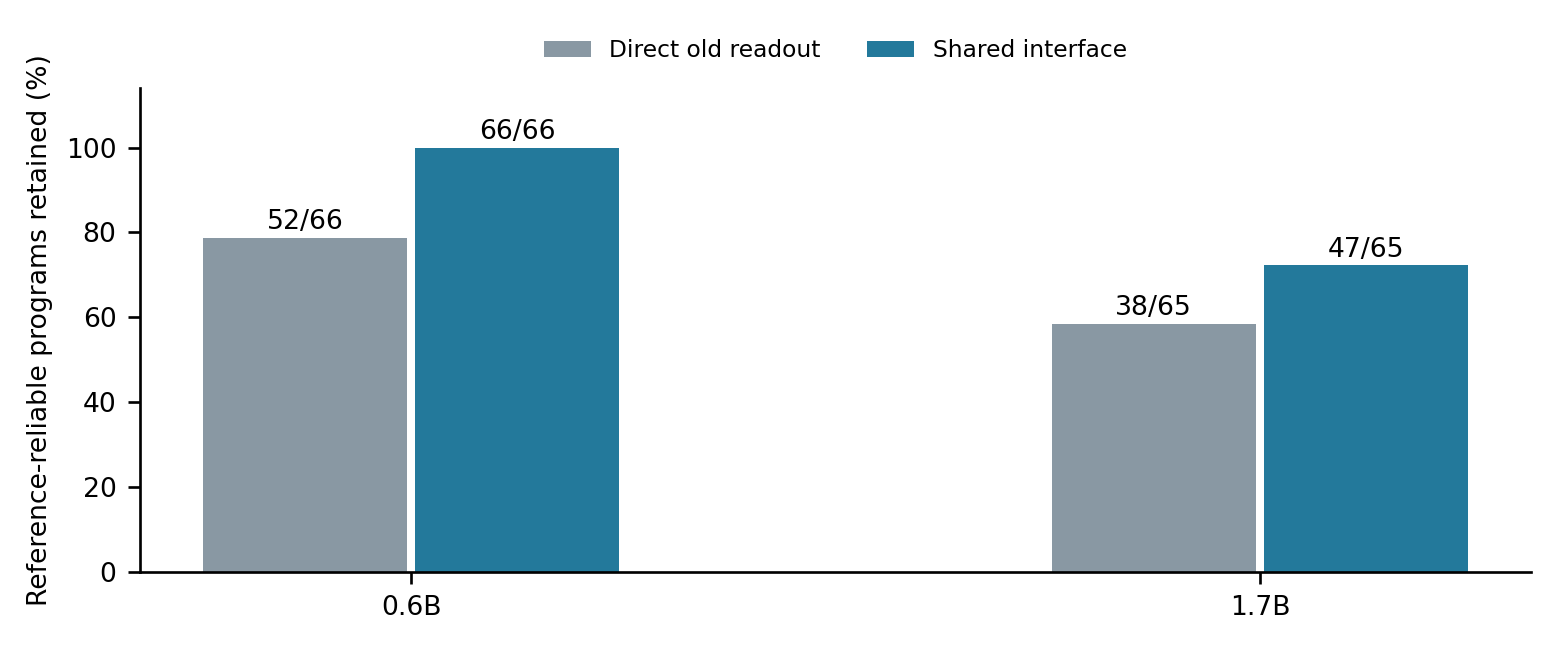
\includegraphics[width=\linewidth]{program-retention.png}
\caption{Fresh-stream retention aggregated by model size. Direct reuse and shared transport use the same old readout weights and target means.}
\end{figure}

\subsection{Two repeated quality gains; heterogeneous average effects}
Two of twelve primary acquired updates improve the nonlinear temporal score in all three blocks while retaining all their reference-reliable old programs. In the 1.7B chart with seed 92002, scores rise from $(5.224,4.559,5.242)$ to $(7.045,6.796,6.896)$: gains of 34.9\%, 49.1\% and 31.6\%. That update exceeds both the same-norm and same-action controls in all three blocks and retains all seven old programs through the interface. Direct reuse retains five.

In the 0.6B chart with seed 96003, score changes are $(+0.188,+0.103,+0.340)$, with all five old programs retained. The matched-action control is stronger in the first two blocks, so this case establishes repeated quality gain and compatibility, rather than control superiority.

\begin{figure}[ht]\centering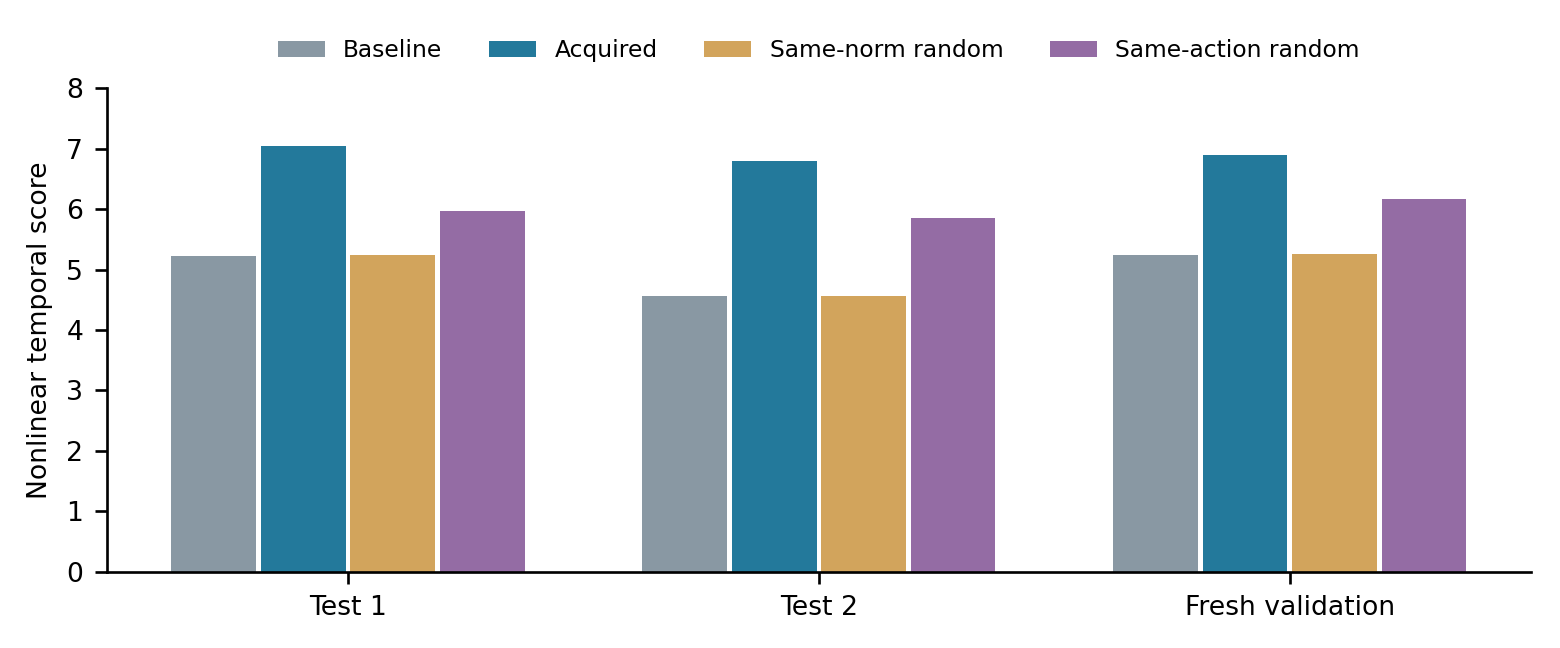
\includegraphics[width=\linewidth]{controlled-example.png}
\caption{The 1.7B, seed-92002 controlled example. This is one specified chart within the complete twelve-chart experiment.}
\end{figure}

The full primary average is negative (Table~\ref{tab:means}). The 1.7B seed-92001 chart loses most of its measured processing quality and retains none of its 18 reference-reliable old programs. Every numeric state remains within the declared bound, so bounded execution alone is insufficient to establish useful computation. A source transport fit with low residual likewise fails to certify fresh-program retention in this case. This localizes the next threshold: acquire a context-sensitive rule that selects or rejects an update based on evidence predictive of later quality and compatibility.

\begin{table}[ht]\centering\small
\begin{tabular}{llrrr}\toprule
Model & Addition & Test 1 & Test 2 & Fresh\\\midrule
0.6B & Acquired & +0.128 & +0.303 & -0.271\\
0.6B & Same-norm random & +0.008 & -0.001 & +0.026\\
0.6B & Same-action random & -0.004 & -0.015 & -0.101\\
1.7B & Acquired & -1.798 & -1.625 & -1.366\\
1.7B & Same-norm random & +0.002 & +0.003 & -0.026\\
1.7B & Same-action random & -1.971 & -1.786 & -1.465\\
\bottomrule\end{tabular}

\caption{Mean score changes over six charts per size for the primary $+2\%$ condition. Blocks 1 and 2 are P59 held-out blocks; block 3 is P60 fresh validation. All arms use the same target suite.}\label{tab:means}
\end{table}

\begin{figure}[ht]\centering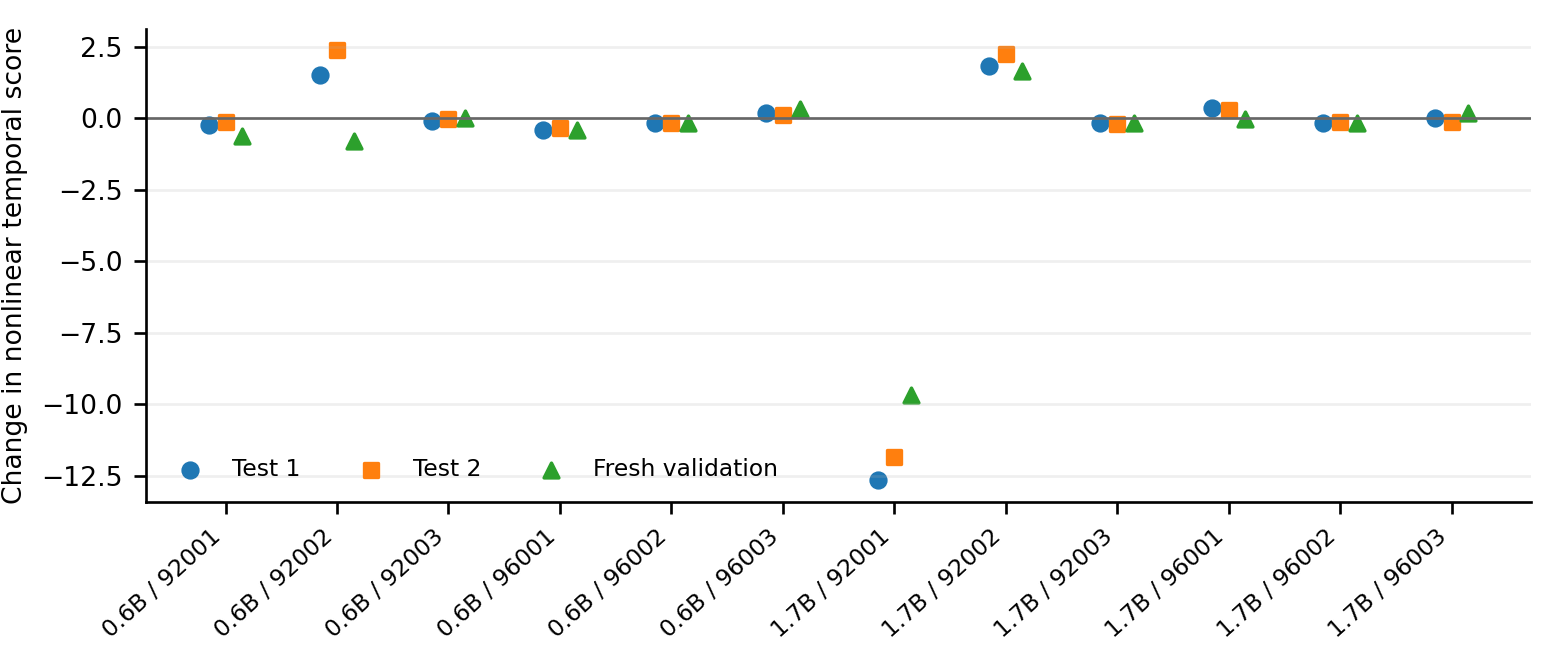
\includegraphics[width=\linewidth]{all-primary-updates.png}
\caption{All primary acquired-update effects. The signed changes and the adverse 1.7B case are retained in the headline evidence.}
\end{figure}

\section{Acquisition and lifecycle ledger}
The deployed return has 16,384 coefficients at 0.6B and 32,768 at 1.7B; augmentation changes their values without expanding that matrix. Recurrent state remains eight-dimensional and the native body is called once per step. Compatibility adds a $40\times40$ float64 matrix (12,800 bytes), 160 serialized normalization values (1,280 bytes), and affine observation work. These additions are charged rather than treated as free preservation.

P59 uses 630,880 native two-position sequences per model, including fresh source acquisition, all doses, controls and padding. P60 uses 73,728 per model. Independent verification adds 2,048 per model: 1,413,312 incremental sequences in total. The inherited source studies contribute a separately reported 834,732 sequences. Pretraining is inherited; electrical energy was not measured. Source trajectories, readout fitting, storage and verification are recorded separately from deployed execution.

\begin{table}[ht]\centering\footnotesize
\begin{tabular}{llrrrr}\toprule
Study & Model & Native sequences & Source/fit s & Whole run s & Peak RSS MiB\\\midrule
P59 & 0.6B & 630,880 & 6.10 & 323.8 & 755.9\\
P59 & 1.7B & 630,880 & 21.31 & 801.4 & 1521.3\\
P60 & 0.6B & 73,728 & 0.04 & 39.6 & 739.5\\
P60 & 1.7B & 73,728 & 0.04 & 95.1 & 1606.3\\
\bottomrule\end{tabular}

\caption{Recorded timing and process-memory measurements. P59 and P60 timings include different work scopes; see the JSON ledger for native-only, source-fit and wall-time fields.}\label{tab:cost}
\end{table}
The model arrays occupy approximately 317 and 914 million bytes in these quantized loads. Whole-process peak RSS reaches approximately 0.79 and 1.68 billion bytes in the recorded runs. A small controller state is therefore not a claim of a correspondingly small whole-process memory footprint. The experiments retain many simultaneous conditions and trajectories for measurement; deployed per-chart state is reported separately.

\section{Building blocks and the contribution}
Orthogonal temporal target families and linear readouts provide an established way to characterize dynamical computation~\cite{dambre}. Input-driven reservoir adaptation, including intrinsic plasticity, already studies how unlabeled experience changes a dynamical substrate~\cite{ip}. Here the frozen model is retained while an external return update changes its recurrent execution.

Pretrained transformers have previously been repurposed across non-language computation tasks with frozen core components and trainable interfaces~\cite{lu}. Model stitching learns alignment layers between fixed neural representations~\cite{stitch}; relative representations and latent-space translation study communication across representation spaces~\cite{relative,translation}. These works supply direct conceptual and technical foundations for shared compatibility. We use ordinary ridge alignment rather than introducing a new linear alignment estimator.

The contribution tested here is a specific joint acquisition protocol: preserve a working return, augment it using source-calibrated response geometry, acquire a single target-label-free observation interface for the changed runtime, and evaluate both new-runtime quality and unchanged-program retention on fresh experience with the costs included. The complete dose/control record distinguishes this mechanism from a claim that all unlabeled updates improve quality. It also exposes a clear next research object: update selection coupled to compatibility prediction, rather than repeated fitting of each old task.

\section{A foundation for the next acquisition cycle}
The public checkpoint answers the paired mechanism question constructively: acquired execution and a reusable compatibility interface can coexist, and one controlled chart exhibits repeated quality improvement with full old-program retention. Across the full experiment, shared transport provides a substantial retention benefit while the fixed update rule has heterogeneous and negative mean quality effects.

The next experiment should learn a context-scoped update policy from neural trajectory evidence, seal that policy before new charts and streams, and test whether it can select beneficial updates while preserving old interfaces. Repeated accepted updates can then test consolidation, retention and net acquisition cost over a sequence rather than one cycle. Those experiments would turn the present executable mechanism into a cumulative capability-acquisition claim. The present finite checkpoint supplies the records, baselines and failure cases needed to make that test informative.

\appendix
\section{Complete primary case record}
\begin{table}[ht]\centering\small
\begin{tabular}{llrrrrr}\toprule
Model & Seed & $\Delta_1$ & $\Delta_2$ & $\Delta_3$ & Direct & Shared\\\midrule
0.6B & 92001 & -0.252 & -0.129 & -0.627 & 5/5 & 5/5\\
0.6B & 92002 & +1.502 & +2.376 & -0.787 & 17/18 & 18/18\\
0.6B & 92003 & -0.096 & -0.037 & +0.002 & 15/16 & 16/16\\
0.6B & 96001 & -0.394 & -0.343 & -0.397 & 4/13 & 13/13\\
0.6B & 96002 & -0.178 & -0.154 & -0.157 & 7/9 & 9/9\\
0.6B & 96003 & +0.188 & +0.103 & +0.340 & 4/5 & 5/5\\
1.7B & 92001 & -12.654 & -11.833 & -9.670 & 0/18 & 0/18\\
1.7B & 92002 & +1.821 & +2.237 & +1.655 & 5/7 & 7/7\\
1.7B & 92003 & -0.178 & -0.187 & -0.157 & 17/19 & 19/19\\
1.7B & 96001 & +0.355 & +0.291 & -0.037 & 4/6 & 6/6\\
1.7B & 96002 & -0.158 & -0.141 & -0.168 & 8/10 & 10/10\\
1.7B & 96003 & +0.024 & -0.116 & +0.181 & 4/5 & 5/5\\
\bottomrule\end{tabular}

\caption{All twelve acquired $+2\%$ updates. $\Delta_k$ is the nonlinear temporal score change in block $k$. Direct and Shared are fresh-stream old-program retention.}
\end{table}
The artifact additionally records all four signed doses and both matched-control families, every functional score, identities of gained/lost targets, source calibration and numerical admissibility. No best-dose selection replaces the primary $+2\%$ result.

\section{Reproduction and evidence integrity}
The checkpoint contains immutable numeric records, source snapshots, protocols, model revisions, receipt hashes, a model-free independent replay and native reproduction entrypoints. Offline verification reconstructs Legendre targets, frozen-readout predictions, source calibration and transport fitting. It reproduces 336 P59 block score vectors and 180 P60 frozen-program score vectors; the largest recorded $R^2$ difference is $6.99\times10^{-10}$ and the transport refit difference is zero. Seventy-six pre-assessment seals verify.

Independent execution through the original checkpoints reproduces 4,032 saved native outputs bit exactly; 4,096 sequences including padding are charged. Loaded-parameter digests agree before and after. File manifests support integrity checks; exact native bit equality is a recorded property of the specified software and hardware configuration, while other platforms should report their numerical tolerances.

The 0.6B model revision is \texttt{173234aa840d113125e9f2271100ddbaf16c9620}; the 1.7B revision is \texttt{21457c6f51ed54a7c16e988c0844db973815c137}. Runners use NumPy 2.5.4, MLX 0.32.4 and MLX-LM 0.32.2 on an Apple M4 Max with 36 GiB memory. Model weights are downloaded separately under their upstream license. The checkpoint guide distinguishes replay of supplied records, re-execution from inherited fixtures and the recorded cost of acquiring those fixtures.

\begin{thebibliography}{10}\raggedright
\bibitem{sg1} N. Oh and P. Attie. Shaping Gap Benchmark: Effect Interfaces for Compositional Execution of Frozen Neural Computation. Repository paper, 2026. \url{https://github.com/calysteon/shaping-gap-benchmark/blob/main/paper/shaping-gap-benchmark.pdf}.
\bibitem{sg2} N. Oh and P. Attie. Shaping Gap Benchmark II: Scalable Effect-Interface Evaluation and Verified Functional Construction. Repository paper, 2026. \url{https://github.com/calysteon/shaping-gap-benchmark/tree/main/checkpoints/02-scaling-and-functions}.
\bibitem{dambre} J. Dambre, D. Verstraeten, B. Schrauwen and S. Massar. Information Processing Capacity of Dynamical Systems. \emph{Scientific Reports} 2, 514, 2012. \url{https://doi.org/10.1038/srep00514}.
\bibitem{ip} B. Schrauwen, M. Wardermann, D. Verstraeten, J. J. Steil and D. Stroobandt. Improving reservoirs using intrinsic plasticity. \emph{Neurocomputing} 71, 1159--1171, 2008. \url{https://biblio.ugent.be/publication/419558}.
\bibitem{lu} K. Lu, A. Grover, P. Abbeel and I. Mordatch. Pretrained Transformers as Universal Computation Engines. 2021. \url{https://arxiv.org/abs/2103.05247}.
\bibitem{stitch} Y. Bansal, P. Nakkiran and B. Barak. Revisiting Model Stitching to Compare Neural Representations. \emph{NeurIPS}, 2021. \url{https://arxiv.org/abs/2106.07682}.
\bibitem{relative} L. Moschella, V. Maiorca, M. Fumero, A. Norelli, F. Locatello and E. Rodol\`a. Relative Representations Enable Zero-Shot Latent Space Communication. \emph{ICLR}, 2023. \url{https://arxiv.org/abs/2209.15430}.
\bibitem{translation} V. Maiorca, L. Moschella, M. Fumero, F. Locatello and E. Rodol\`a. Latent Space Translation via Inverse Relative Projection. 2024. \url{https://arxiv.org/abs/2406.15057}.
\bibitem{qwen} Qwen Team. Qwen3 Technical Report. 2025. \url{https://arxiv.org/abs/2505.09388}.
\end{thebibliography}
\end{document}
